\section{Backtesting Framework}
\label{sec:backtesting-framework}

Stockrium includes a historical simulation subsystem for evaluating whether the analytical pipeline behaves consistently with its intended decision rules. The subsystem is designed as an engineering and research tool rather than an automated trading facility. It reuses the production multi-agent components and mirrors the technical scoring conditions in a vectorized historical engine, applies explicit execution assumptions, and produces machine-readable artifacts for later evaluation. Experimental results obtained from this framework are reported in Chapter~6.

Established Python frameworks already provide reusable data feeds, strategy lifecycles, order simulation, indicators, portfolio accounting, and fast parameter exploration. For example, Backtrader provides an event-driven strategy and broker abstraction \cite{backtraderDocs2026}, while VectorBT emphasizes vectorized analysis over pandas and NumPy objects \cite{vectorbtDocs2026}. Stockrium nevertheless implements a focused simulator because the object being evaluated is not only a conventional deterministic trading strategy. Each historical candidate must reconstruct a date-bounded production request, invoke the same specialist agents and structured aggregator used by the application, enforce Stockrium-specific confidence and veto rules, compare the agent-filtered result with an engine-only branch, and return artifacts through the existing FastAPI and Supabase workflow.

Adapting a general framework would still require custom adapters for historical agent state, language-model outputs, source-availability markers, the scoring-parity gate, and Stockrium's stored result schema. A compact in-project framework makes these assumptions visible and allows exact correspondence with the production decision path to be tested. The trade-off is that mature frameworks provide broader execution, portfolio, optimization, and broker features that the current simulator does not reproduce. Thus, the custom implementation is justified by production-path fidelity and experimental traceability, not by a claim that general frameworks are inadequate; cross-checking future deterministic results with an established engine remains desirable.

The implementation is exposed through the access-controlled internal \texttt{POST} \path{/api/agentic/backtest} endpoint. A request specifies the stock symbol, historical boundaries, minimum technical score, maximum holding period, optional score-based exit, and automatic or manual evidence selection. Historical OHLCV data are loaded through the market service, while VN-Index candles provide the reference series for regime analysis. Each completed run returns parity results, model decisions, simulated trades, metrics, benchmark comparisons, statistical tests, and visualization data.

\subsection{Evaluation Architecture}
\label{subsec:backtest-evaluation-architecture}

The backtest reuses the production specialist-agent and aggregator implementations together with a vectorized historical indicator and scoring engine, rather than maintaining a separate research-only prediction model. Figure~\ref{fig:backtest-execution-flow} shows the execution path. Daily candles first pass through the deterministic historical engine. Only dates on which the combined score crosses the configured threshold become candidates for multi-agent analysis. A candidate is admitted as a trade only when the final structured recommendation is \textit{Mua} (Buy). The engine-only baseline retains all technical candidates, allowing the filtering effect of the complete multi-agent pipeline to be isolated.

\begin{figure}[H]
    \centering
    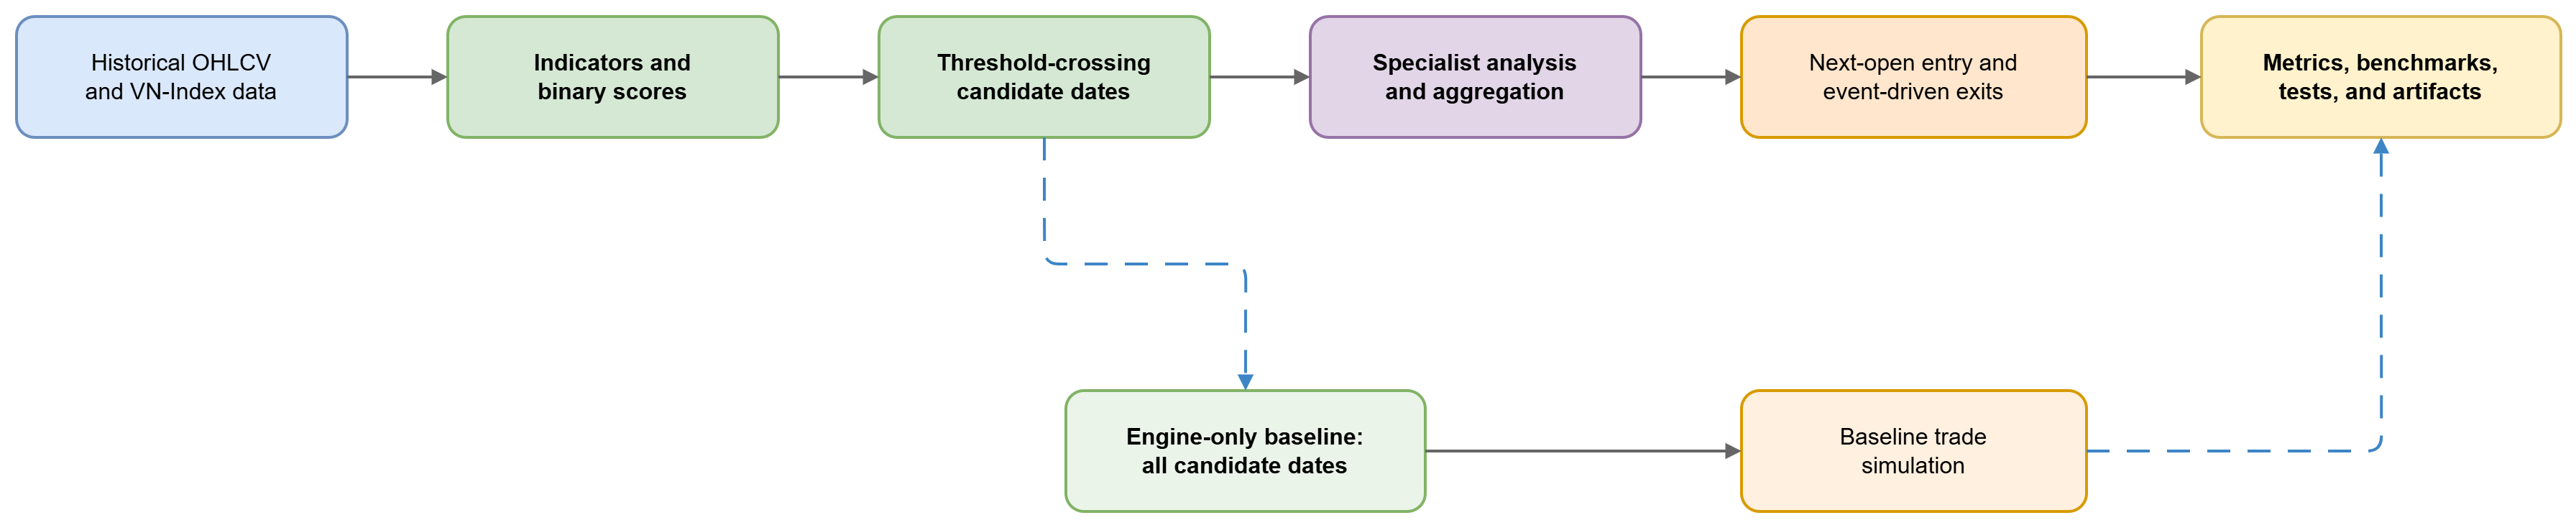
\includegraphics[width=\textwidth,keepaspectratio]{diagrams/chapter4/stockrium_backtesting_flow.png}
    \caption{Execution flow of the Stockrium backtesting framework}
    \label{fig:backtest-execution-flow}
\end{figure}

Before a full experiment runs, the system performs a scoring-parity gate. Ten candle indices are sampled between the end of the 50-candle warm-up and the final observation. At each sample, the technical agent is restricted to data ending on that date and explicitly directed to use the backtest indicator source; its scores are then compared with the vectorized scoring engine. A run is rejected unless the match rate is 100\%. This verifies that the node-level and vectorized scoring rules agree when they consume the same historical-engine output. It does not compare the numerical indicators produced by the live application service with those produced by the backtest engine, and it does not by itself establish profitability.

\subsection{Technical Signal Construction}
\label{subsec:backtest-signal-construction}

The historical indicator engine calculates the same five nominal indicator families and periods described in Section~\ref{subsubsec:technical-analysis-agent}: RSI with a 14-period lookback, SMA20 and SMA50, 20-period Bollinger Bands at two standard deviations, MACD $(12,26,9)$, and KDJ with a 9-period range and 3-period smoothing. As noted in Section~\ref{subsec:technical-analysis-foundations}, some numerical conventions currently differ from the live application service. Each perspective contributes either zero or one point, giving a combined score $s_t\in[0,5]$ when all indicators are enabled.

The first 50 observations form the warm-up interval because SMA50 is the longest rolling feature. With default threshold $\tau=3$, a candidate is emitted only when the score enters the qualified region,

\begin{equation}
    \mathrm{candidate}_t =
    \mathbb{I}\!\left(s_t \geq \tau \;\land\; s_{t-1}<\tau\right).
    \label{eq:backtest-threshold-crossing}
\end{equation}

The crossing rule avoids opening a new candidate on every day of a persistent high-score interval. The last candle is never signaled because no next-candle execution price exists. Model-backed analysis is invoked only on candidate dates, reducing the number of language-model calls. Technical and article plans use the candidate date as their upper boundary and a 252-day lookback in the main daily experiment.

Equation~\ref{eq:backtest-threshold-crossing} is an author-defined Stockrium event rule rather than a signal formula taken from an external strategy. It converts the implemented binary technical score into one candidate only when the score newly enters the qualified region; the threshold is an exposed experiment parameter.

\subsection{Trade Simulation and Cost Model}
\label{subsec:backtest-trade-simulation}

The simulator is long-only and permits at most one open position per symbol. A signal completed after candle $t$ is entered at the open of candle $t+1$, avoiding execution at the same close used to construct the signal. Structured entry, take-profit, stop-loss, and maximum-holding values supplied by the aggregator are used after validity checks; otherwise, the next open and configured holding limit are applied.

Starting with the entry candle, the daily low is checked against the stop-loss level and the daily high against the take-profit level. Stop loss is evaluated first, giving a conservative outcome when both levels fall within one daily bar and intraday order is unavailable. If configured, a score below three schedules a \texttt{SIGNAL\_EXIT} at the following open. Otherwise, a position exits at the final permitted close with reason \texttt{TIMEOUT}. The scan resumes after the exit, so same-symbol positions do not overlap.

The default transaction cost is $c=0.0015$, or 0.15\% per side. For entry price $P_k^{\mathrm{in}}$ and exit price $P_k^{\mathrm{out}}$, net return is

\begin{equation}
    r_k = \frac{P_k^{\mathrm{out}}-P_k^{\mathrm{in}}}{P_k^{\mathrm{in}}}-2c.
    \label{eq:backtest-net-trade-return}
\end{equation}

The default round-trip deduction is therefore 0.30\%. The simulation does not separately model bid--ask spread, market impact, partial fills, taxes, price-limit queues, or gap slippage. These assumptions are considered when interpreting the experimental results.

Equation~\ref{eq:backtest-net-trade-return} is the framework's accounting definition of simulated net trade return. The value $c=0.0015$ is a configurable modeling assumption per side, not a claim that every Vietnamese investor incurs one universal statutory fee. Keeping it explicit allows later experiments to replace it with broker-, tax-, liquidity-, or period-specific costs.

\subsection{Measures, Benchmarks, and Artifacts}
\label{subsec:backtest-metrics-tests}

The framework reports trade count, win rate, average and median trade return, total compounded return, annualized return, maximum drawdown, a trade-level Sharpe statistic, Calmar ratio, profit factor, and exit counts. Total return and the post-trade equity sequence are

\begin{equation}
    R_{\mathrm{total}}=\prod_{k=1}^{K}(1+r_k)-1,
    \qquad
    E_k=\prod_{j=1}^{k}(1+r_j).
    \label{eq:backtest-total-return}
\end{equation}

Let $H_k=\max_{j\leq k}E_j$ denote the running peak. Maximum drawdown is the minimum of $(E_k-H_k)/H_k$. The implemented Sharpe statistic is

\begin{equation}
    S=\sqrt{K}\frac{\overline{r}}{s_r},
    \label{eq:backtest-sharpe}
\end{equation}

where $s_r$ is the sample standard deviation of trade returns. It follows the risk-adjusted comparison principle of the Sharpe ratio \cite{sharpe1994ratio}, but is scaled by trade count rather than a fixed annual frequency. It is therefore an internal comparison statistic rather than a conventional annualized portfolio Sharpe ratio.

Equation~\ref{eq:backtest-total-return} and the stated maximum-drawdown calculation are implementation definitions based on geometric compounding of sequential trade returns and decline from the running equity peak. Equation~\ref{eq:backtest-sharpe} is explicitly adapted from Sharpe's risk-adjusted comparison principle, with the nonstandard $\sqrt{K}$ trade-count scaling identified above. Stating these origins separates standard financial concepts from Stockrium-specific event, cost, and scaling choices.

The evaluation suite compares the full pipeline with the engine-only strategy, buy-and-hold exposure, and 1,000 random-entry simulations. It also provides a one-sample $t$-test, sign-permutation test, score--return information coefficient, confidence grouping, rolling walk-forward windows, and VN-Index regime analysis. Because repeated strategy comparisons can overfit historical data \cite{bailey2017pbo}, the framework retains negative and non-significant results instead of reporting only successful securities.

Each run produces visualization JSON containing prices, indicators, decisions, entries, exits, and metrics. The artifact can be served by FastAPI and uploaded to Supabase Storage. A separate aggregate JSON file is updated per symbol to support VN30-level analysis. Chapter~6 uses these saved artifacts as the quantitative evidence for evaluation.
